\documentclass[11pt]{beamer}
\usetheme{Frankfurt}
\usecolortheme{rose}

\usepackage{hyperref}
\usepackage{url}
\usepackage{graphicx}
\usepackage{amsmath,amsthm, amssymb, latexsym}
\usepackage[english]{babel}
\usepackage{epstopdf}
\usepackage{color}
\usepackage{bm}

\usefonttheme{professionalfonts}

\DeclareMathOperator*{\argmax}{arg\,max}
\DeclareMathOperator*{\argmin}{arg\,min}

\newcommand{\citecolor}[1]{({\color{blue} #1})}
\def\E{\mathbb{E}}

\newcommand\blfootnote[1]{%
  \begingroup
  \renewcommand\thefootnote{}\footnote{#1}%
  \addtocounter{footnote}{-1}%
  \endgroup
}

%Gummi|063|=)

\title[CLGP]{Deep Reinforcement Learning: Tic-Tac-Toe }
\author[Liang]{Kevin Liang}
\institute[Duke University]{Duke University}
\date{02 July 2016}
\begin{document}

\begin{frame}
\maketitle
\end{frame}



%%%%%%%%%%%%%%%%%%%%%%%%%%%%%%%%%%%%%%%%%%%%%%%%%%%%%%%
\section{Introduction}

\begin{frame}{Introduction}
	\begin{itemize}
	
		\item Goal: Have an agent learn how to play Tic-tac-Toe using deep reinforcement learning 
		\item Tic-Tac-Toe game
		\begin{itemize}
			\item Players X and O take turns placing marks on a 3x3 grid
			\item Player that achieves a 3-in-a-row wins
			\item If the board fills up without a winner: draw
		\end{itemize}
		\item Toy example to get started before tackling more complicated settings (eg. Atari games of OpenAI Gym)
		
	\end{itemize}
\end{frame}

\section{Methods}
\begin{frame}{Deep Reinforcement Learning Agent Set-up}
	\begin{minipage}[t]{0.45\linewidth}
		\begin{itemize}
			\item Agent is given a 125x125 image of the state of the board, not the 3x3 state space directly.
			\item Agent not informed of rules. Does not know:
				\begin{itemize}
					\item what leads to a win/loss
					\item own identity
					\item marking an already occupied spot is an illegal move
				\end{itemize}
			\item Perform weight updates using RL algorithm:
			\begin{itemize}
				\item Policy Gradients
				\item Q-Learning
			\end{itemize}
		\end{itemize}
	\end{minipage}%
	\hfill
	\begin{minipage}[t]{0.45\linewidth}
		\centering
		\begin{figure}[tttDL]
			\centering
			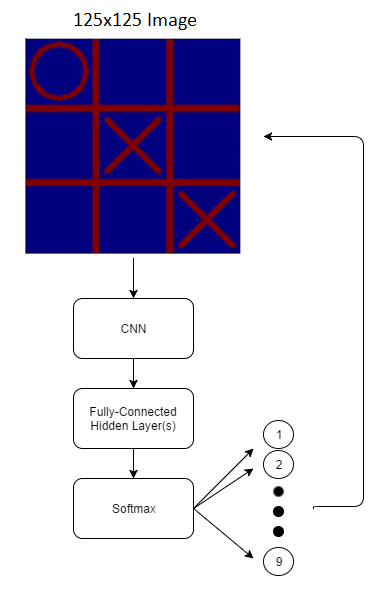
\includegraphics[width=.95\textwidth]{Figures/deeptictactoe.png}
		\end{figure}
	\end{minipage}
	
\end{frame}

\begin{frame}{Optimal opponent}
	\begin{itemize}
		\item Newell and Simon Tic-Tac-Toe Rules:
		\begin{itemize}
			\item Rule 1: If agent can win, then make a 3-in-a-row
			\item Rule 2: If opponent can win, block the winning move
			\item Rule 3: Make a fork (two 2-in-a-rows)
			\item Rule 4: Block an opponent's fork, while simultaneously making a 2-in-a-row if possible
			\item Rule 5: Take the center
			\item Rule 6: If opponent has a corner, take the opposite corner
			\item Rule 7: Take an empty corner
			\item Rule 8: Take an empty side
		\end{itemize}		
		\item Add a "difficulty" parameter that controls how often the "optimal" agent makes a random move, instead of always following rules
		\begin{itemize}
			\item Allows for the deep RL agent to occasionally win (and therefore learn)
		\end{itemize}	
	\end{itemize}
\end{frame}

\section{Questions}
\begin{frame}{Questions}
	\begin{itemize}
		\item CNN architecture details
		\item Hyperparameters (CNN and RL)
		\item Computer/GPU/cluster to train it on
	\end{itemize}
\end{frame}


\end{document}
